\chapter{Desarrollo teórico}
En este capítulo proveeremos con la base matemática. Principalmente nos basaremos en los libros \textit{Advanced Data Analysis
from an Elementary Point of View}\cite{ada} y \textit{Probabilistic Networks for Practitioners — A
Guide to Construction and Analysis of Bayesian
Networks and Influence Diagrams}\cite{pgm}, junto con el capítulo \textit{An overview of the representation and 
discovery of causal relationships using bayesian networks}\cite{cooper}.

\section{Introducción a las redes bayesianas}
Las redes bayesianas nos ayudan a modelar y entender las muchas variables que informan nuestro proceso de 
toma de decisiones. Las decisiones más complejas están normalmente basadas en una multitud de factores o 
variables. Por ejemplo, imaginemos que el dueño de un equipo de fútbol tiene que decidir antes del comienzo 
de cada temporada cuánto dinero hay que invertir en nuevos jugadores. Habrá de considerar los ingresos 
probables por las ventas de jugadores no deseados; el gasto neto relativo de otros
equipos; y el posible impacto negativo en el desempeño del equipo de hacer demasiados cambios de personal de una 
vez, entre otros. Podemos mapear la decisión que tiene que hacer, y todas las diferentes variables, usando 
una red bayesiana, esto es, un modelo gráfico que captura la relación entre variables que están bajo 
supuestos de causalidad o influencia.\cite{things-to-know-BN}

Básicamente entonces, \textbf{una red bayesiana es un diagrama que 
usa flechas o arcos dirigidos para mostrar cómo distintos factores, representados por nodos elípticos, se 
influencian los unos a los otros.} Cada nodo viene con su tabla de probabilidad, la cual refleja las 
posibilidades de varios desenlaces, provenientes de las influencias que le afectan directamente. Una vez 
la estructura del grafo y la tabla de una red han sido definidos, hay algoritmos estándar que 
calculan los estados de las variables desconocidas basándose en los estados de las variables conocidas en el
modelo.\cite{learning-algorithms-BN-comparison}, \cite{BN-achilles-heel}, \cite{different-algorithmic-schemes}

Una de las razones por las que las redes bayesianas son tan potentes es que pueden realizar inferencias 
tanto predictivas como diagnósticas. Por ejemplo, podemos por un lado predecir la posición en la liga de un equipo para 
un valor dado (observación) de rendimiento, y por otro ingresar un estado de posición en la 
liga como observación para examinar qué nivel de desempeño del equipo podría explicarla. Estos algoritmos estándar son
llamados algoritmos de "propagación bayesiana"\cite{Cano2004},\cite{more-algorithms}, \cite{back-prop} porque se basan en el teorema de Bayes, en el que la 
probabilidad de una variable desconocida se actualiza después de que se obtenga evidencia relevante para esa variable.\cite{prop-alg}

\section{Grafos}
Un grafo es un par $G = (V, E)$, donde $V$ es un conjunto finito de vértices distinguibles y 
$E \subseteq V \times V$ es un conjunto de aristas. Un par ordenado $(u, v) \in E$ denota un borde dirigido
del vértice $u$ al vértice $v$, y se dice que $u$ es padre de $v$ y $v$ hijo de $u$.
El conjunto de padres e hijos de un vértice $v$ se denotará por $pa(v)$ y $ch(v)$, respectivamente.
Como veremos más adelante, según lo que representen, los vértices se muestran como círculos 
etiquetados, óvalos o polígonos, los bordes dirigidos como flechas, y los 
bordes no dirigidos como líneas.

\begin{figure}[h!]
    \centering
    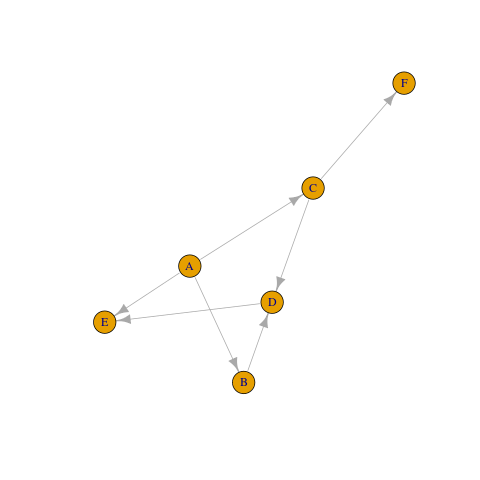
\includegraphics[width=\textwidth]{../img/dag.png}
    \caption{Grafo dirigido acíclico con ocho vértices y ocho aristas dirigidas, donde, por ejemplo, el vértice 
    etiquetado $E$ tiene dos padres etiquetados $T$ y $L$. Las etiquetas de los vértices se 
    refieren a los nombres de los vértices, los nombres de las variables representadas por 
     los vértices, o etiquetas descriptivas asociadas a las variables representadas por los vértices.}
    \label{img:dag1}
\end{figure}
    
Se usa la notación $u$ $\underrightarrow{G}$ $v$ para denotar $(u,v) \in E$, o simplemente 
$u \rightarrow v$ si se sobreentiende $G$. Si $(u,v) \in E$ y $(v,u) \in E$, la arista 
entre $u$ y $v$ es no dirigida, y se denota ${u,v} \in E$ o $u - v$. Se usará la notación 
$u ~ v$ para denotar $u \rightarrow v$ , $u \leftarrow v$, o $u - v$. Los vértices $u$ y $v$ 
se dicen que están conectados en G si



\section{Probabilidades} 

\section{Redes probabilísticas}
Las redes probabilísticas son modelos gráficos de interacciones (causales) entre una
conjunto de variables, donde las variables se representan como vértices (también: nodos)
de un gráfico y las interacciones (dependencias directas) como aristas dirigidas (también:
enlaces y arcos) entre los vértices. Cualquier par de vértices no conectados indican 
independencia (condicional) entre las variables representadas
por estos vértices en circunstancias particulares que se pueden leer fácilmente desde el
grafico. Por lo tanto, las redes probabilísticas capturan un conjunto de dependencia (condicional)
y propiedades de independencia asociadas con las variables representadas en el
la red.

Los gráficos han demostrado ser un lenguaje muy intuitivo para representar
tales declaraciones de dependencia e independencia, y por lo tanto proporcionan una excelente
lenguaje para comunicar y discutir las relaciones entre las 
variables del dominio del problema, las cuales se pueden representar de forma muy compacta 
mediante gráficos dirigidos acíclicos (DAG).

Los gráficos de cadena son una generalización de los DAGs, capaces de representar un espectro más amplio de 
clases de dependencia y supuestos de independencia. El poder expresivo añadido
viene, sin embargo, con el coste de un aumento significativo en la complejidad semántica, 
lo que hace que la especificación de los factores de probabilidad conjunta sea mucho menos intuitiva.
Por ello, los modelos de gráficos en cadena han ganado muy poca
popularidad como modelos prácticos para los sistemas de soporte de decisiones, y vamos a
concentrarnos exclusivamente en modelos que factoricen de acuerdo con los DAG.

Las redes probabilísticas pueden verse como representaciones compactas de reglas de causa-efecto "difusas" 
que, contrariamente a los sistemas normales basados en reglas, son capables de realizar tanto razonamiento 
deductivo y abductivo, como intercausal. El razonamiento deductivo o causal
sigue la dirección de los vínculos causales que hay entre las variables de un modelo; por ejemplo, al saber
que un paciente sufre de angina podemos concluir con alta probabilidad que
el paciente tiene fiebre y dolor de garganta. Por otro lado, el razonamiento abductivo o diagnóstico 
va en contra de la dirección de los nexos causales; por ejemplo, observar
que un paciente tiene dolor de garganta proporciona evidencia de que anginas es un diagnóstico correcto.

Sin embargo, la propiedad que distingue a la inferencia en redes probabilísticas
de otros paradigmas de razonamiento automático es su capacidad para hacer razonamientos intercausales: 
obtener evidencia que apoye una sola hipótesis (o un subconjunto de
hipótesis) conduce a la disminución de la creencia en las otras con las que compiten y para las que no se 
han encontrado unas bases que las soporten. 

\section{Redes causales}

\section{Resolución de redes probabilísticas}

